\documentclass{article}

% Use the neurips_2023 style
\usepackage[preprint, nonatbib]{neurips_2024}
\usepackage[square,numbers]{natbib}
\bibliographystyle{abbrvnat}

% to compile a preprint version, e.g., for submission to arXiv, add add the
% [preprint] option:
%\usepackage[preprint]{neurips_2023}

% to compile a camera-ready version, add the [final] option, e.g.:
%\usepackage[final]{neurips_2023}

% to avoid loading the natbib package, add option nonatbib:
%\usepackage[nonatbib]{neurips_2023}

\usepackage[utf8]{inputenc} % allow utf-8 input
\usepackage[T1]{fontenc}    % use 8-bit T1 fonts
\usepackage{hyperref}       % hyperlinks
\usepackage{url}            % simple URL typesetting
\usepackage{booktabs}       % professional-quality tables
\usepackage{amsfonts}       % blackboard math symbols
\usepackage{nicefrac}       % compact symbols for 1/2, etc.
\usepackage{microtype}      % microtypography
\usepackage{xcolor}         % colors
\usepackage{graphicx}
\usepackage{amsmath}
\usepackage{amssymb}
\usepackage{enumitem}
\usepackage{subcaption}

\title{TilePilot: A Lightweight Framework for Optimizing GPU Kernels}

\author{%
  Jack Le\\
  Stanford University\\
  \texttt{jackle@stanford.edu} \\
  \And
  Nathan Paek\\
  Stanford University\\
  \texttt{nathanjp@stanford.edu} \\
  \And
  William Li\\
  Stanford University\\
  \texttt{willyli@stanford.edu} \\
}

\begin{document}

\maketitle

\begin{abstract}
High-performance GPU kernel development remains a critical bottleneck in machine learning systems, requiring deep expertise in parallel programming and hardware optimization. While recent work has shown that large language models (LLMs) can generate functional GPU kernels, existing approaches rely on expensive brute-force sampling strategies costing up to \$15 per kernel. We present TilePilot, a lightweight framework that automatically translates PyTorch operators into efficient TileLang \cite{tilelang2025} kernels through knowledge retrieval and mathematical reasoning. Our approach bootstraps from 37 hand-written kernels to generate 214 verified kernels across KernelBench's \cite{ouyang2025kernelbenchllmswriteefficient} first three difficulty levels, containing 250 problems total. We achieve significantly higher success rates than baselines while reducing generation costs compared to contemporary approaches. On a held-out test set of 100 additional problems, TilePilot demonstrates strong generalization with 72 successful kernels and a mean speedup of 1.25x over PyTorch baselines. Notably, our system not only translates operations but also acts as an LLM compiler, discovering optimizations that reduce asymptotic complexity in several cases.
\end{abstract}

\section{Background and Setup}

\subsection{Problem Definition}

GPU kernel optimization represents a fundamental challenge in high-performance computing and machine learning. Writing efficient CUDA or GPU kernels requires extensive expertise in parallel programming, memory hierarchy optimization, and hardware-specific tuning—skills that are scarce and expensive to develop.

\textbf{Inputs and Outputs:} Our system takes PyTorch neural network operations (e.g., matrix multiplication, convolution, element-wise operations) as input and produces functionally equivalent TileLang kernel implementations as output. TileLang \cite{tilelang2025} is a domain-specific language built on Apache TVM that provides structured scheduling primitives for GPU kernel development.

\textbf{Goals and Constraints:} We aim to generate kernels that satisfy three core constraints: (1) \textit{Functional correctness}—the generated TileLang kernel must produce identical results to the original PyTorch operation across all valid inputs; (2) \textit{Performance competitiveness}—the kernel should achieve reasonable performance compared to PyTorch's optimized implementations; and (3) \textit{Cost efficiency}—the generation process must be economically practical for large-scale deployment.

\textbf{Research Question:} Can retrieval-augmented generation and composition produce functionally correct and performant GPU kernels in a low-resource domain-specific language more efficiently and cost-effectively than brute-force sampling methods?

The fundamental difficulty of this problem lies in the intersection of two challenges: the complexity of GPU kernel optimization and the scarcity of training data for domain-specific languages. More specifically, we face the following challenges:

\textbf{Limited Training Data:} TileLang is a DSL that was released in late April 2025, roughly six weeks ago, with very minimal official examples and low representation in existing code repositories, creating a severe distribution gap for pre-trained models.

\textbf{Performance Sensitivity:} Unlike general programming where functionality is often sufficient, GPU kernels require sophisticated understanding of memory access patterns, thread scheduling, and hardware utilization to achieve acceptable performance.

\textbf{Economic Constraints:} Existing approaches like Sakana AI's CUDA Engineer \cite{sakana2024} rely on expensive trial-and-error sampling, generating thousands of candidates at approximately \$15 per successful kernel, which is prohibitively expensive for our use case.

The core insight driving our approach is that GPU kernel optimization often involves recombining known patterns rather than inventing entirely novel algorithms. This observation suggests that knowledge retrieval and composition may be more effective than pure generation for this domain.

\section{Approach}

\subsection{Progressive Learning Framework}

Our approach employs a three-stage progressive learning strategy designed to bootstrap from minimal examples to a comprehensive kernel generation system:

\textbf{Stage 1: Seed Generation.} We manually implemented 37 high-quality TileLang kernels covering fundamental operations including matrix multiplication, vector operations, and reductions. These kernels serve dual purposes: they provide the initial knowledge base for retrieval and establish patterns for the LLM to learn from. Each kernel includes detailed annotations explaining the mapping from PyTorch operations to TileLang constructs.

\textbf{Stage 2: Knowledge Retrieval.} We implement a retrieval-augmented generation system using DSPy \cite{dspy2023} that treats our growing kernel collection as a dynamic knowledge base. For each generation request, the system embeds the target PyTorch operation and retrieves the $k=5$ most semantically similar existing kernels based on cosine similarity in the embedding space. These retrieved kernels serve as contextual examples for the LLM.

\textbf{Stage 3: Performance Optimization.} For kernels that compile correctly but exhibit suboptimal performance, we employ structured multi-turn conversations where the LLM analyzes potential bottlenecks across four categories: workload imbalance, redundant computation, memory bandwidth limitations, and algorithmic inefficiencies.

\subsection{RAG-Enhanced Generation Process}
Our pipeline generates optimized TileLang kernels through a four-stage process using DSPy \cite{dspy2023}:

\textbf{Query Processing:} We analyze the input PyTorch operation to extract key semantic features. This includes identifying the operation type and its mathematical properties, analyzing input/output tensor shapes and strides, understanding computational patterns and dependencies, and examining memory access patterns and data locality. These features form the foundation for finding relevant optimization patterns.

\textbf{Similarity Retrieval:} We compute embeddings for both the query and our kernel knowledge base. The retrieval system employs cosine similarity to identify semantically related kernels, considering both structural and functional similarities. This approach ensures we retrieve the most relevant examples that share common optimization patterns with the target operation.

\textbf{Context Construction:} Retrieved kernels are transformed into structured examples that map PyTorch operations to equivalent TileLang primitives. Each example highlights key optimization patterns and scheduling decisions, along with performance metrics and implementation notes. This structured context enables the LLM to understand both the functional requirements and optimization opportunities.

\textbf{Generation:} The LLM synthesizes a new kernel by adapting relevant patterns from retrieved examples, composing optimized subroutines, and applying domain-specific optimizations. We then evaluate the performance of the generated kernel against the KernelBench \cite{ouyang2025kernelbenchllmswriteefficient} validation suite and store the results in our knowledge base.

This approach is grounded in the observation that GPU kernel optimization typically involves recombining and adapting established techniques rather than inventing entirely new algorithms. By leveraging our knowledge base of verified kernels, we enable efficient pattern reuse while maintaining the flexibility to handle novel optimization scenarios.

\subsection{Performance Optimization}
Our performance optimization process employs a two-step approach that combines bottleneck analysis with targeted kernel optimization, using DSPy \cite{dspy2023} for each step.

\textbf{Step 1: Bottleneck Analysis.} Given a kernel implementation and its current performance metrics, our system performs a comprehensive bottleneck analysis across four key dimensions:

\begin{itemize}
    \item \textbf{Memory Bandwidth:} Analyzes memory access patterns, coalescing, and bank conflicts
    \item \textbf{Computational Efficiency:} Evaluates arithmetic intensity and redundancy
    \item \textbf{Parallelism:} Assesses thread utilization, workload balance, and occupancy
    \item \textbf{Algorithmic:} Identifies opportunities for operator fusion and reduction patterns
\end{itemize}

We further enhance this analysis by retrieving relevant optimization examples from our knowledge base to provide context-aware suggestions.

\textbf{Step 2: Kernel Optimization.} Using the bottleneck analysis and optimization suggestions, along with TileLang guidelines, the system generates an optimized kernel implementation. We then evaluate the performance of the kernel against KernelBench, and repeat the process until the kernel reaches the target speedups or the maximum number of iterations is reached.

\subsection{Case Study: 29\_Matmul\_Mish\_Mish}

To illustrate our optimization process, we present a case study of the 29\_Matmul\_Mish\_Mish kernel, which performs a matrix multiplication followed by two Mish activations. The initial implementation used a suboptimal linear kernel and used the existing PyTorch Mish function, resulting in a speedup of 0.324x. Through iterative optimization, we achieved a final speedup of 1.19x.

\textbf{Initial Optimization:} Given the initial implementation, the model observed that it may be able to gain a speedup by generating an efficient kernel that combined the two Mish operations. This resulted in a speedup of 0.493x.

\textbf{Final Optimization:} Our bottleneck analysis model provided detailed optimization suggestions that guided the implementation. For the matrix multiplication, it recommended using TileLang's optimized T.copy primitive for parallelized memory transfers, implementing double buffering with 3 pipeline stages, and fusing the Mish operations directly into the matrix multiplication epilogue. The result was a single fused kernel for the entire sequence. This resulted in a speedup of 1.19x.

This optimization process demonstrates the effectiveness of our two-pass optimization approach in identifying and addressing performance bottlenecks. However, we observed that the cost of running this system was much higher than the previous system, since it required multiple model calls for each step, repeating until it succeeds. We were only able to run this system on a small subset of kernels as a proof of concept. We hope to explore this approach in more depth in the future.

\section{Evaluation and Results}

\subsection{Definition of Success}

Our research investigates whether retrieval-augmented generation (RAG) can outperform traditional sampling-based approaches for low-resource domain-specific language (DSL) generation. We evaluate success across three key dimensions:

\textbf{Generation Success Rate:} The proportion of PyTorch operations that are successfully translated into functionally correct TileLang kernels, validated through KernelBench's \cite{ouyang2025kernelbenchllmswriteefficient} comprehensive test suite.

\textbf{Cost Efficiency:} The average monetary cost required to generate a single successful kernel, measured in terms of LLM API usage costs.

\textbf{Performance Competitiveness:} The relative performance of our generated kernels compared to their PyTorch baseline implementations, measured in terms of execution speed.

\subsection{Experimental Setup}

\textbf{Benchmark Suite:} We conduct our evaluation using KernelBench \cite{ouyang2025kernelbenchllmswriteefficient}, a diverse benchmark containing 250 GPU kernel optimization tasks categorized into three progressive difficulty levels:
\begin{itemize}
\item \textbf{Level 1:} 100 basic operations (element-wise operations, simple reductions)
\item \textbf{Level 2:} 100 intermediate tasks (operator fusion, memory optimization patterns)
\item \textbf{Level 3:} 50 advanced optimization challenges (multi-kernel fusion, full models)
\end{itemize}

Additionally, we evaluated our approach on a held-out test set of 100 problems acquired from the KernelBench authors, which was not used during system development or for knowledge base construction, providing an unbiased assessment of generalization capabilities.

\textbf{Hardware:} All experiments were conducted on NVIDIA H100 GPUs using Modal. Performance measurements were averaged over 100 trials with warm-up iterations to ensure stable results.

\textbf{Generation Approaches:} We evaluate three distinct approaches to kernel generation:
\begin{itemize}
\item \textbf{Naive Prompting:} Using OpenAI's o3 with only TileLang documentation as context
\item \textbf{Few-shot ICL:} In-context learning utilizing 5 carefully selected diverse examples
\item \textbf{TilePilot (RAG):} Our proposed approach using retrieval-augmented generation with a knowledge base of optimization patterns
\end{itemize}

\textbf{Evaluation Metrics:} We assess functional correctness through KernelBench's validation suite, measure performance using speedup ratios relative to PyTorch implementations, and calculate the cost of each generation attempt.

\subsection{Generation Success Rates}

\begin{figure}[htbp]
    \centering
    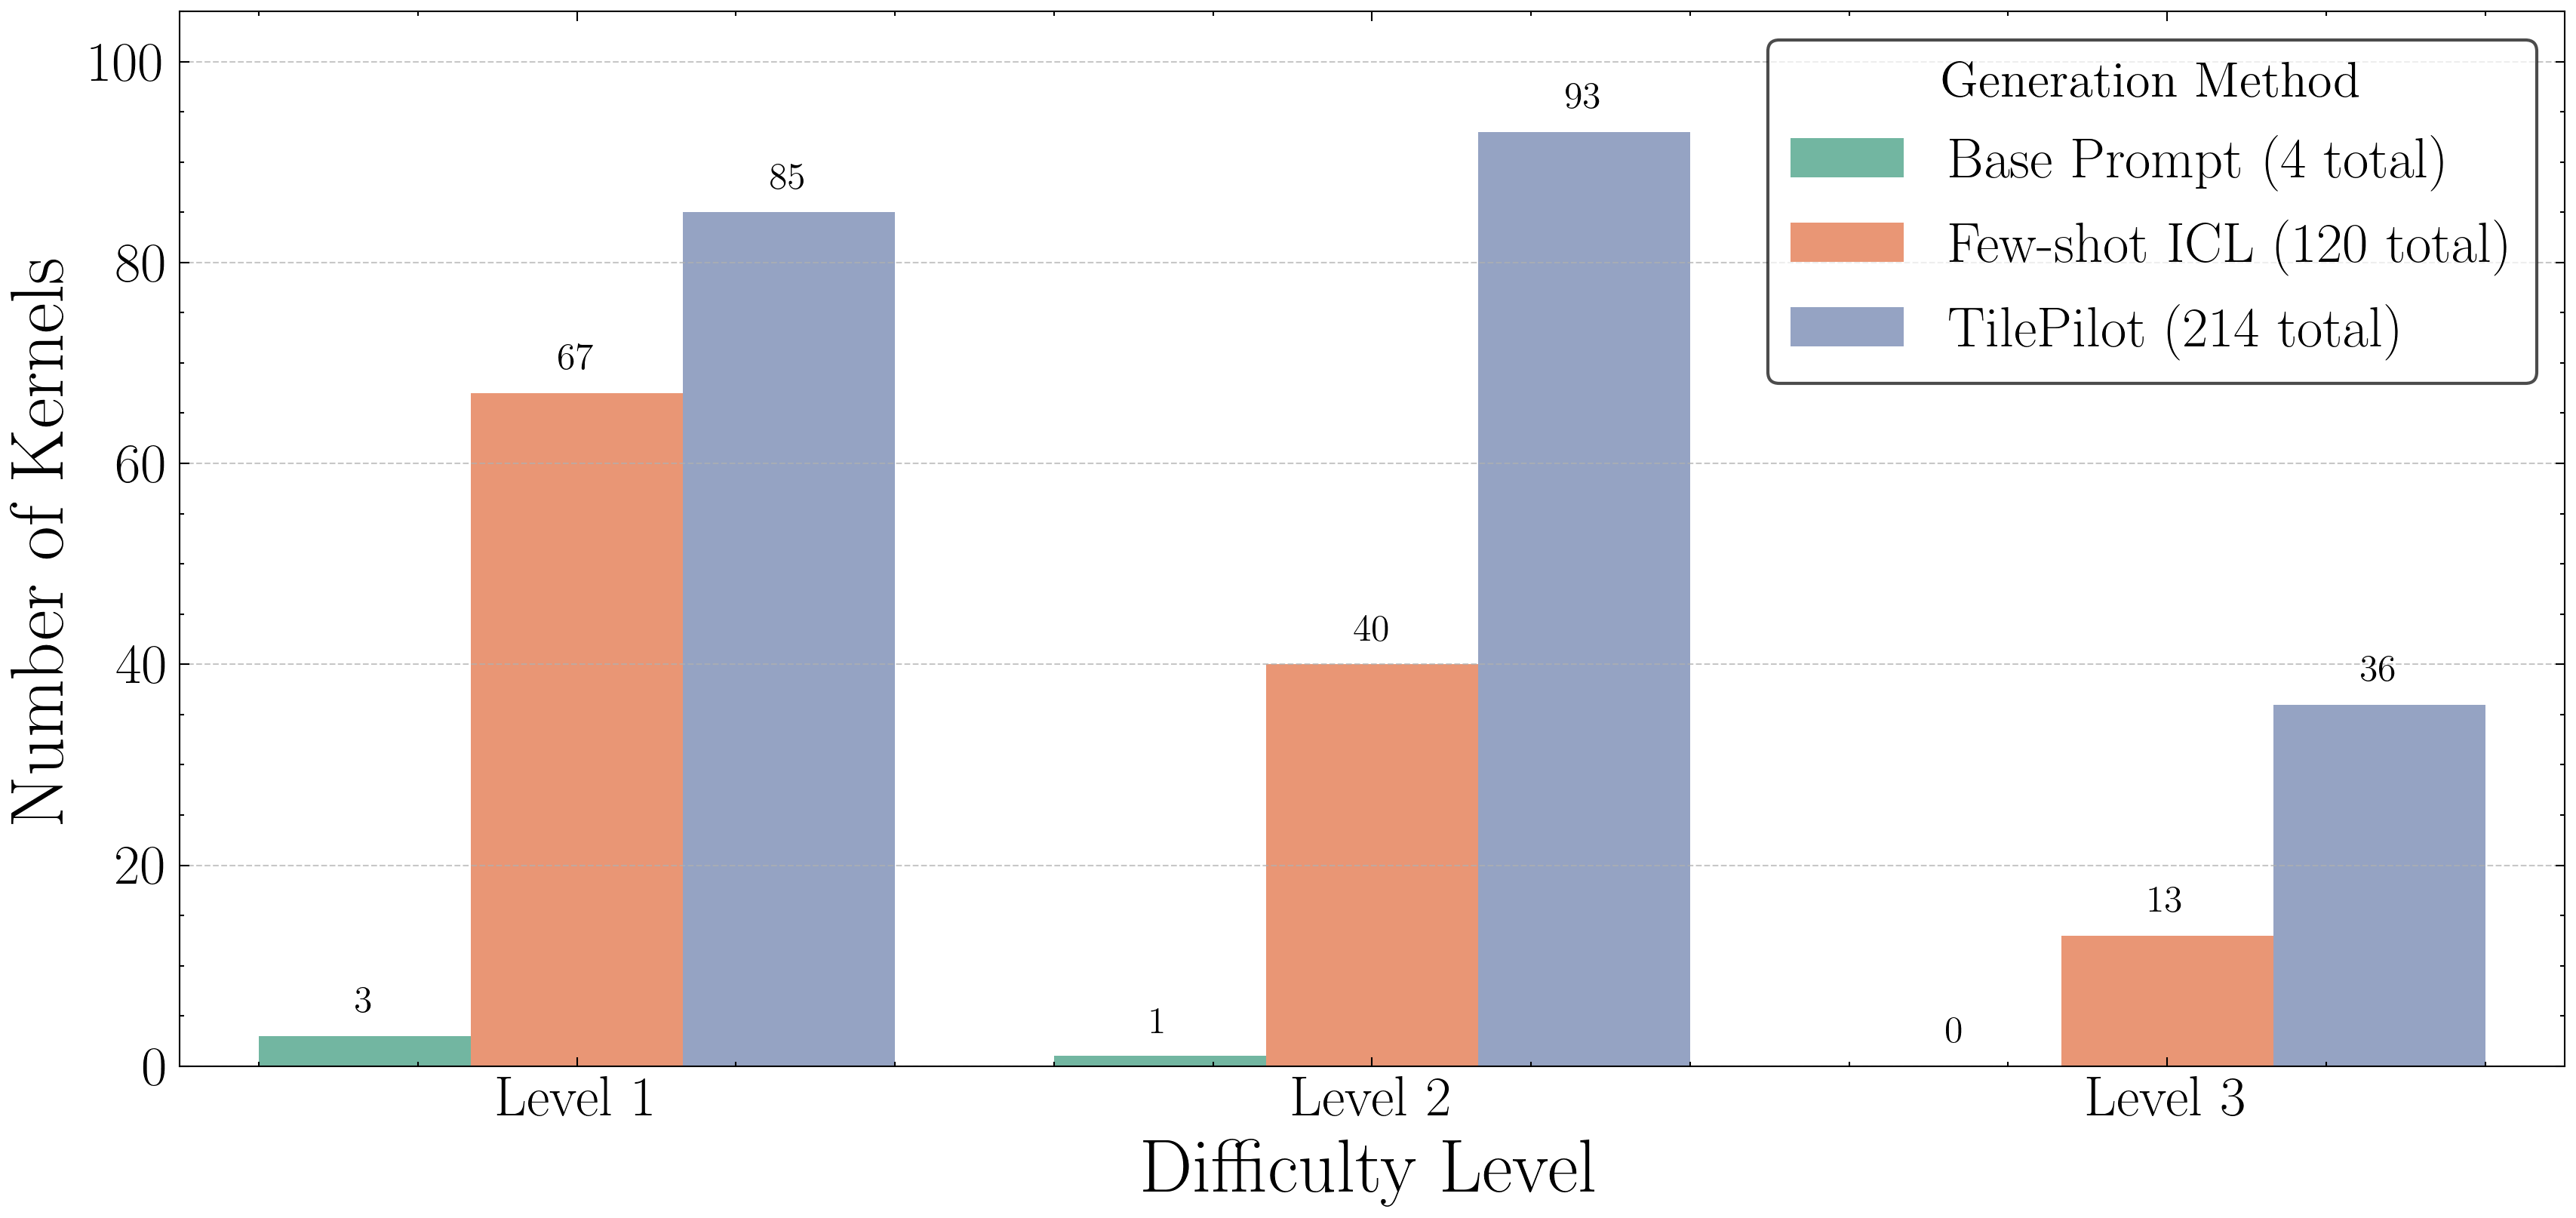
\includegraphics[width=0.8\textwidth]{plots/kernel_success_rate.png}
    \caption{Success rates across levels for different generation approaches. TilePilot (RAG) shows significant improvements over both naive prompting and few-shot ICL, particularly on Level 2 tasks.}
    \label{fig:success_rates}
\end{figure}

Figure \ref{fig:success_rates} presents our core findings on generation success rates across difficulty levels. The results strongly support our hypothesis that RAG can dramatically improve generation success rates. TilePilot successfully generates 214 kernels compared to 120 kernels generated by few-shot ICL, achieving a 78\% relative improvement. Most striking is the 133\% improvement on Level 2 tasks, which aligns with our theory that problems primarily involving operator fusion and lifting benefit the most from our pattern recombination approach.

\subsection{Cost Efficiency Analysis}

Our approach achieves remarkable cost efficiency compared to other approaches. On the tail end of the spectrum, Sakana AI's approach \cite{sakana2024} costs upwards of \$15.00 per successful kernel due to their brute force iterative sampling approach. The naive few-shot ICL approach costs \$0.62 per successful kernel, primarily due to the fact that the prompt needed to be much longer in order to be able to reliably generate a diverse range of kernels. In comparison, TilePilot (RAG) costs \$0.30 per successful kernel, while still achieving a higher success rate than the naive few-shot ICL approach.

\subsection{Performance Analysis}

\paragraph{Distributional Insights} To understand the performance characteristics of our generated kernels, we graph the distribution of speedup ratios compared to PyTorch baselines. Figure~\ref{fig:overall_speedup} shows the overall distribution of speedup ratios (on a log scale) for all generated kernels, while Figure~\ref{fig:speedup_distributions} breaks down the distributions for Level 1 and Level 2 tasks.

\begin{figure}[htbp]
    \centering
    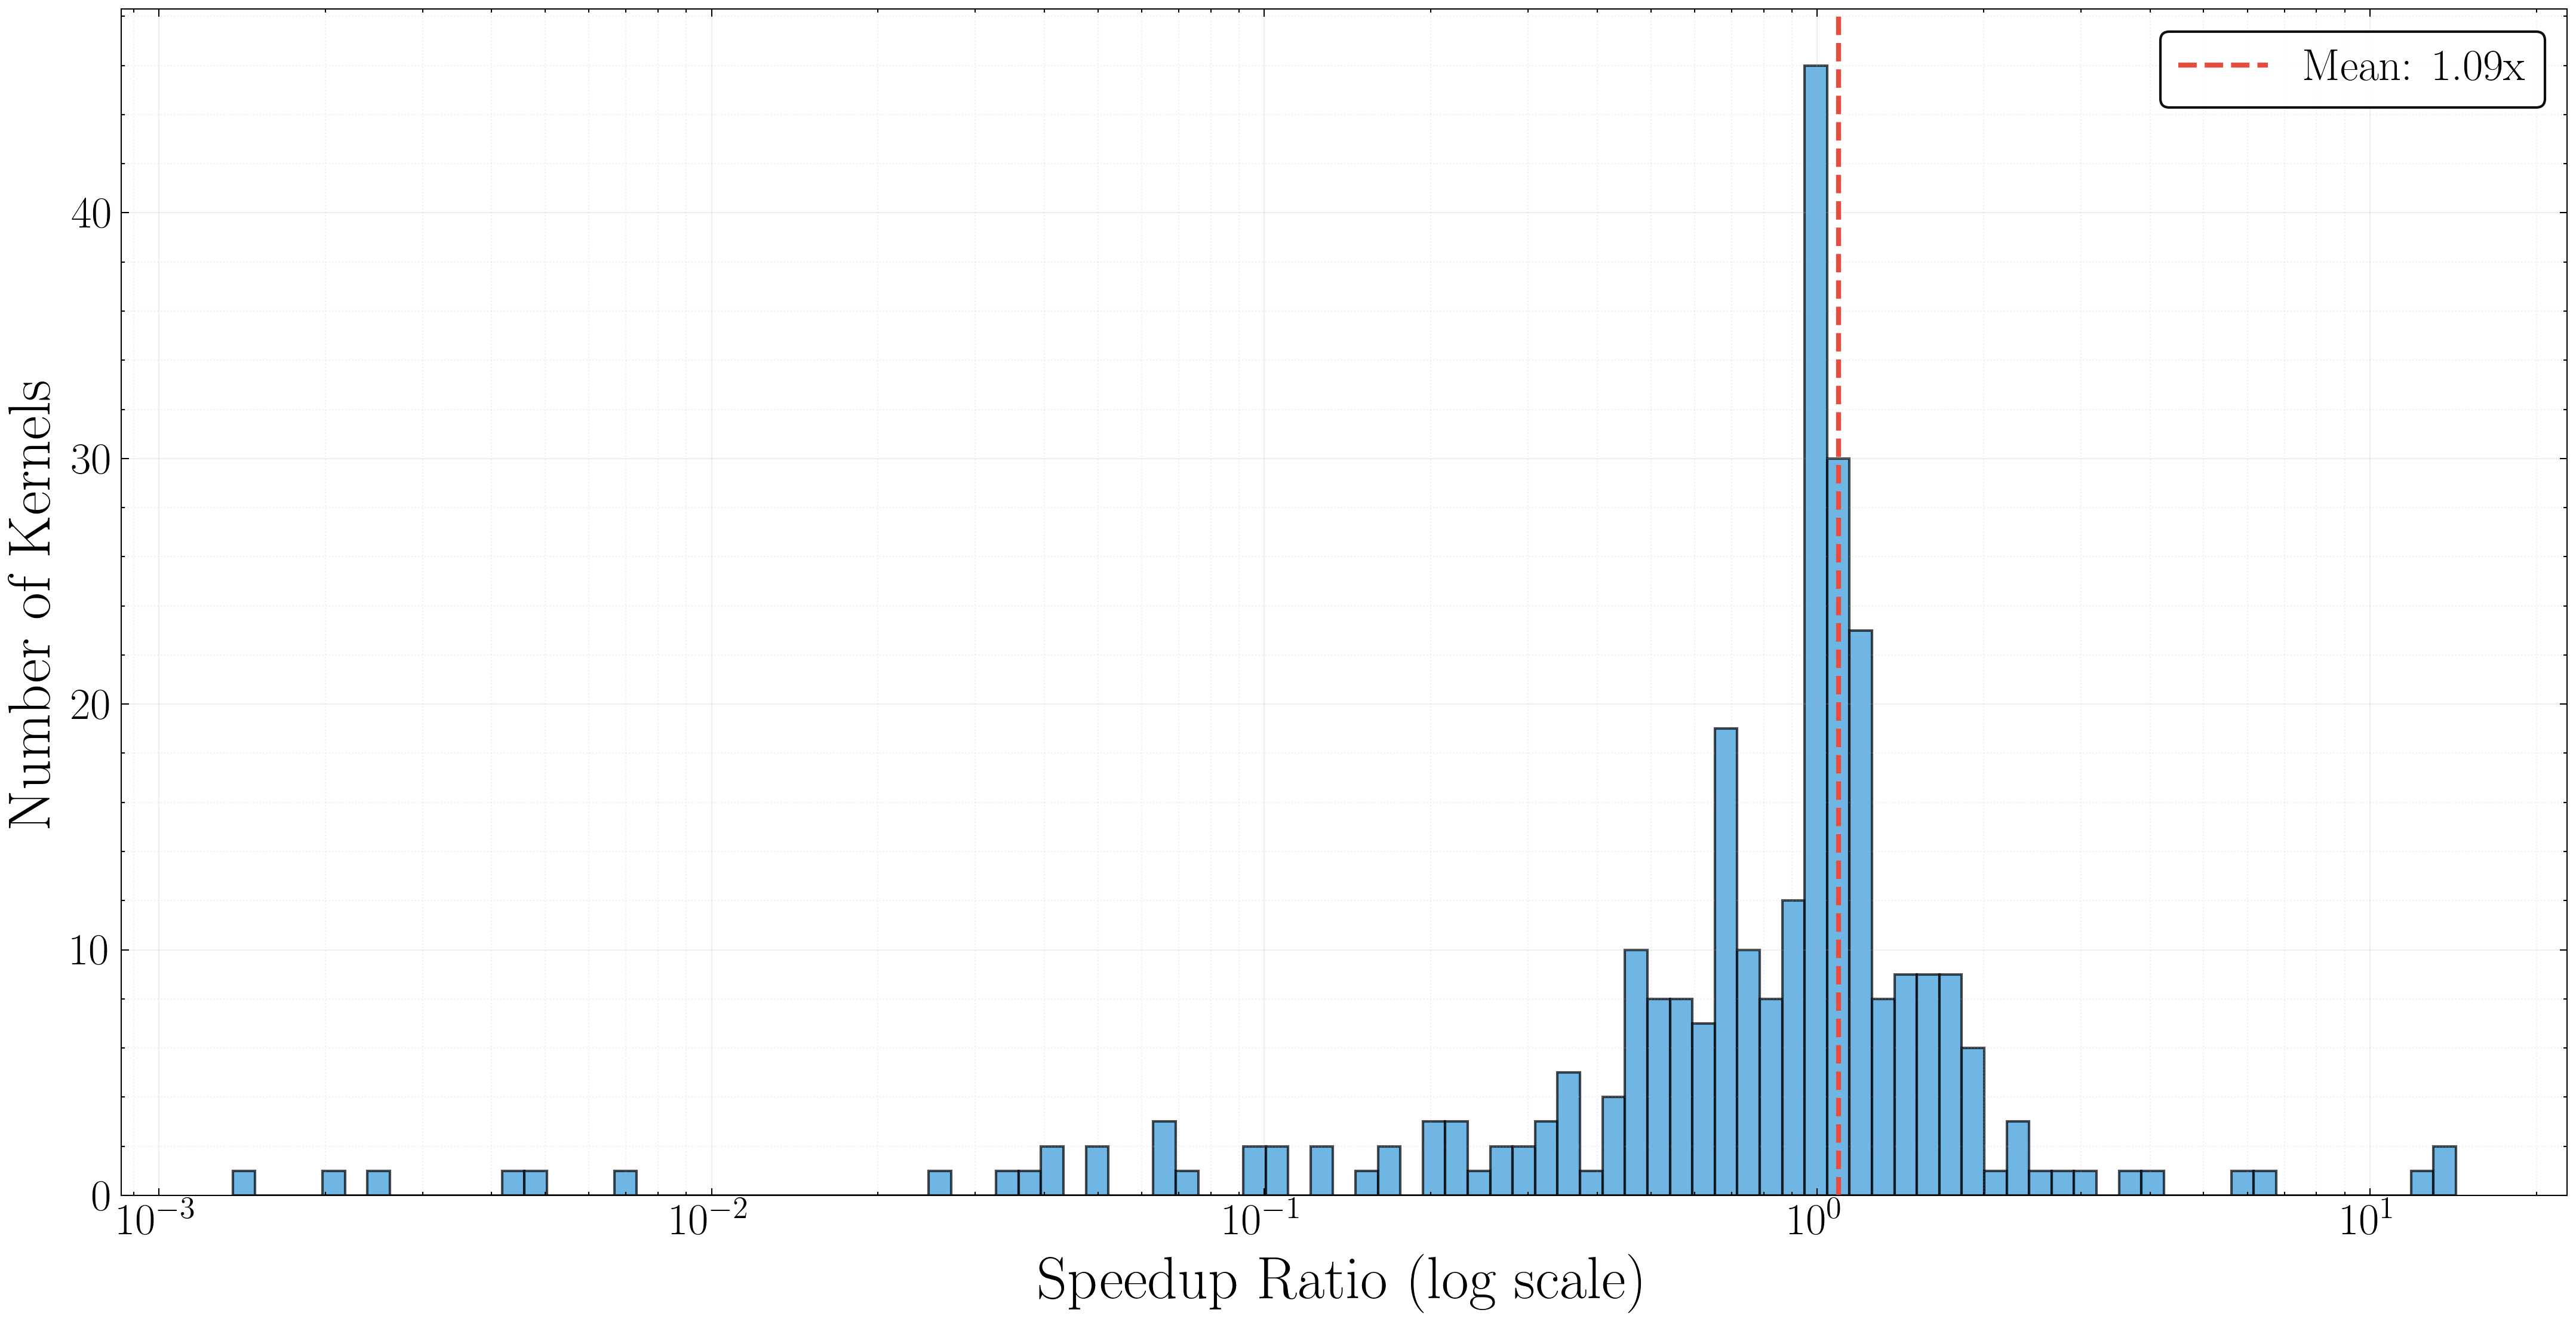
\includegraphics[width=0.8\textwidth]{plots/speedup_distribution_overall.png}
    \caption{Distribution of speedup ratios (log scale) for generated kernels across all difficulty levels.}
    \label{fig:overall_speedup}
\end{figure}

\begin{figure}[htbp]
    \centering
    \begin{subfigure}[b]{0.48\textwidth}
        \centering
        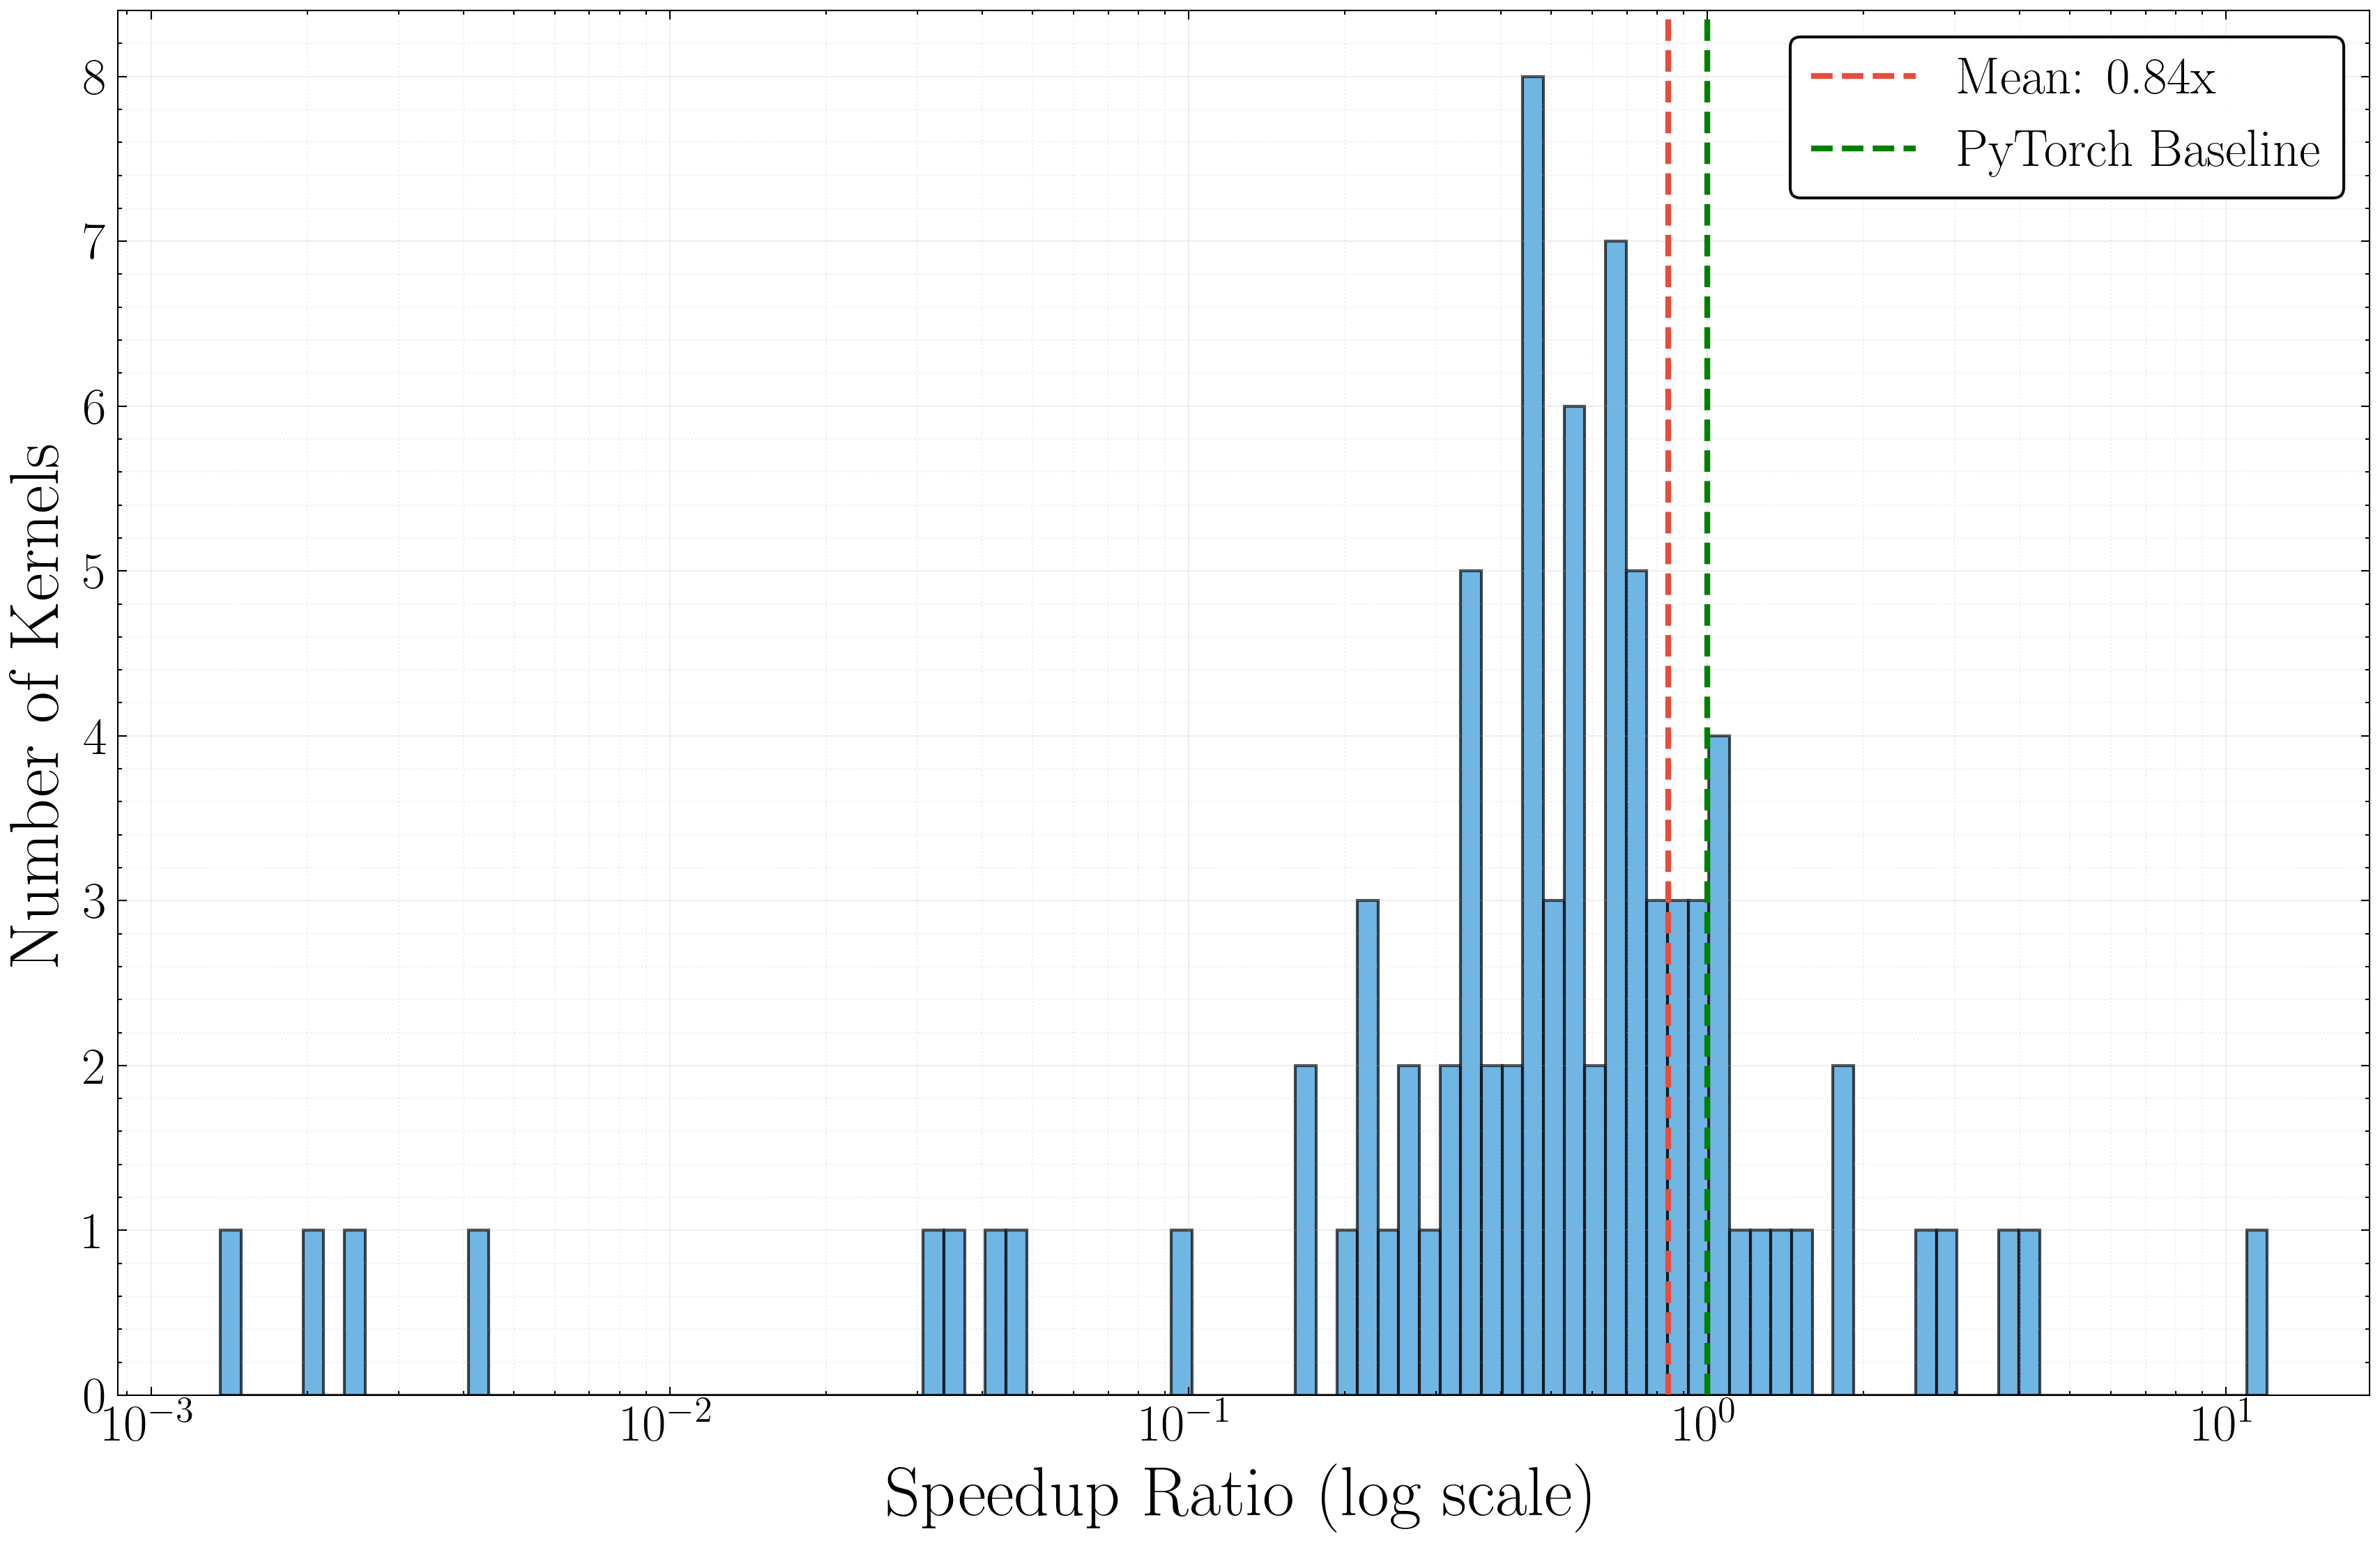
\includegraphics[width=\textwidth]{plots/speedup_distribution_Level1.png}
        \caption{Distribution of speedup ratios for Level 1 kernels.}
        \label{fig:level1_speedup}
    \end{subfigure}
    \hfill
    \begin{subfigure}[b]{0.48\textwidth}
        \centering
        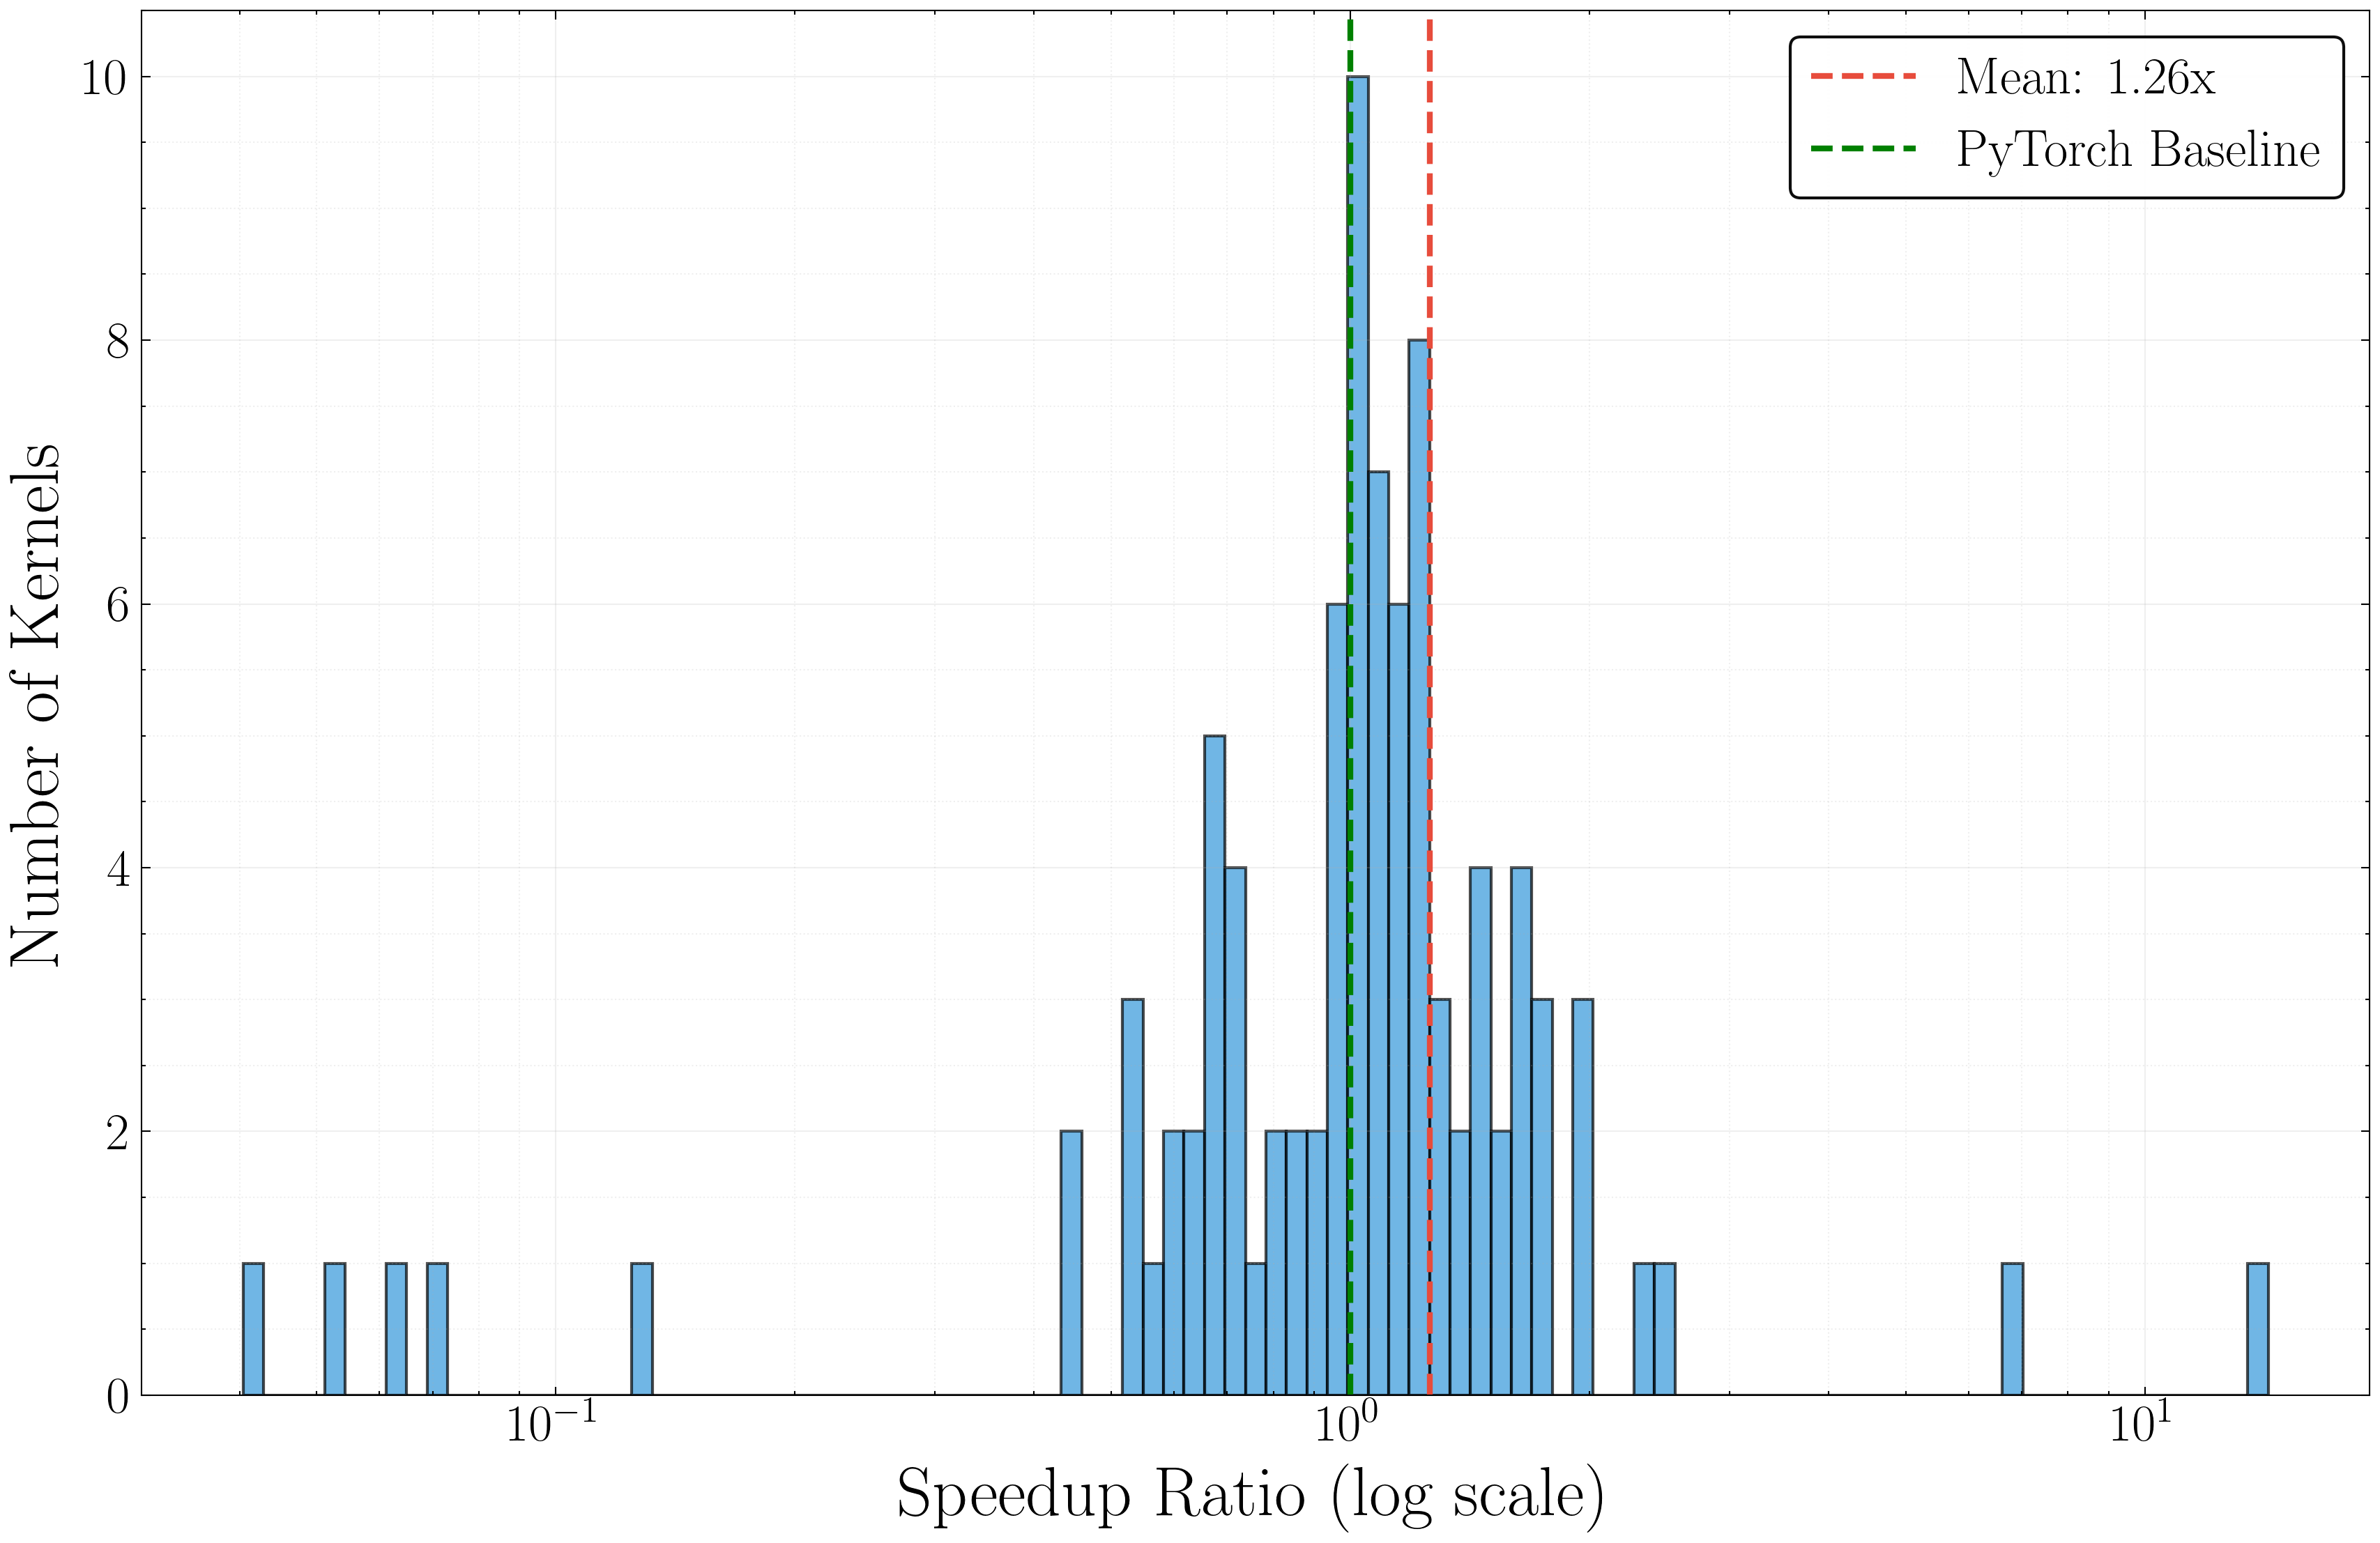
\includegraphics[width=\textwidth]{plots/speedup_distribution_Level2.png}
        \caption{Distribution of speedup ratios for Level 2 kernels.}
        \label{fig:level2_speedup}
    \end{subfigure}
    \caption{Performance distribution (log scale) across difficulty levels. The red vertical line in each plot indicates the mean speedup for that level, and the PyTorch Baseline is marked for reference.}
    \label{fig:speedup_distributions}
\end{figure}
The log-scale in Figures~\ref{fig:overall_speedup} and~\ref{fig:speedup_distributions} allows us to more clearly visualize both high and low performing kernels. The overall distribution (Figure~\ref{fig:overall_speedup}) is largely centered: a significant amount of kernels are within 1x of the PyTorch baseline, with some kernels significantly outperforming.

Breaking down by difficulty, Level 1 kernels (Figure~\ref{fig:level1_speedup}) are tightly clustered slightly below the baseline, with only a small fraction achieving notable speedups. This is expected, as Level 1 tasks are fundamental operations where PyTorch's highly optimized kernels are difficult to outperform. In contrast, Level 2 kernels (Figure~\ref{fig:level2_speedup}) are centered above the baseline, with a substantial number of kernels achieving significant speedups. This supports our hypothesis that pattern recombination and operator fusion are the core strengths of our approach, and are most beneficial for intermediate-complexity tasks compared to elementary operations.

\paragraph{Quantitative Summary}
Table~\ref{tab:performance} summarizes the key statistics for each difficulty level. Our performance analysis reveals notable variations across difficulty levels, with Level 2 kernels demonstrating the most impressive results: 58\% outperform their PyTorch baselines, achieving an average speedup of 1.26x and a maximum observed speedup of 14.3x. This success validates our hypothesis regarding the effectiveness of pattern recombination for operator fusion tasks.

Level 1 and Level 3 kernels show more modest gains, with only 18\% and 25\% exceeding baseline performance, respectively. We believe that the lower performance of Level 1 kernels is due to the fact that for these basic operators, the PyTorch kernels are already highly optimized (in fact, we argue that Level 1 is harder to optimize for than Level 2 in KernelBench, as supported by the KernelBench leaderboard \cite{kernelsseum2024}). The overall average speedup across all kernels is 1.09x, demonstrating consistent performance improvements. The subpar performance for Level 3 suggests there is room for improvement in our approach, as it primarily consists of full models that require complex multi-kernel optimizations.
\begin{table}[h]
\centering
\caption{Performance analysis of generated kernels. ``Kernels $>$ 1.0x'' indicates the number and percentage of kernels that outperform PyTorch.}
\label{tab:performance}
\begin{tabular}{lccc}
\toprule
\textbf{Level} & \textbf{Average Speedup} & \textbf{Maximum Speedup} & \textbf{Kernels $>$ 1.0x} \\
\midrule
Level 1 & 0.84x & 12.0x & 15/85 (18\%) \\
Level 2 & 1.26x & 14.3x & 54/93 (58\%) \\
Level 3 & 0.85x & 5.71x & 9/36 (25\%) \\
\textbf{Overall} & \textbf{1.09x} & \textbf{14.3x} & \textbf{78/214 (36\%)} \\
\bottomrule
\end{tabular}
\end{table}

\paragraph{Comparison to KernelBench Leaderboard}
We compare TilePilot's performance against the current KernelBench leaderboard \cite{kernelsseum2024}. To contextualize this result, we highlight a fundamental difference: leaderboard solutions are written in CUDA, a mature language with extensive representation in LLM training data and decades of optimization research. In contrast, TilePilot generates kernels in TileLang, a DSL released only six weeks prior to our work with very minimal training data availability. The fact that our low-resource DSL approach achieves comparable or superior performance demonstrates the effectiveness of our approach. Table~\ref{tab:leaderboard_comparison} shows this comparison across all levels.
\begin{table}[h]
\centering
\caption{Comparison between TilePilot (TileLang) and KernelBench leaderboard (CUDA) results.}
\label{tab:leaderboard_comparison}
\begin{tabular}{lcccccccc}
\toprule
& \multicolumn{4}{c}{\textbf{TilePilot}} & \multicolumn{4}{c}{\textbf{Leaderboard}} \\
\cmidrule(lr){2-5} \cmidrule(lr){6-9}
\textbf{Level} & \textbf{Total} & \textbf{Mean} & \textbf{Max} & \textbf{Speedup $>$ 1.0x} & \textbf{Total} & \textbf{Mean} & \textbf{Max} & \textbf{Speedup $>$ 1.0x} \\
\midrule
Level 1 & 85 & 0.84x & 12.0x & 18\% & 65 & 0.88x & 13.22x & 20\% \\
Level 2 & 93 & 1.26x & 14.3x & 58\% & 65 & 1.18x & 7.08x & 52\% \\
Level 3 & 36 & 0.85x & 5.71x & 25\% & 26 & 0.82x & 1.32x & 15\% \\
\bottomrule
\end{tabular}
\end{table}


Despite CUDA's resource advantages, TilePilot demonstrates competitive performance across all levels. For Level 2 tasks, our approach exceeds CUDA performance with higher average speedups (1.26x vs 1.18x) and more kernels beating PyTorch (58\% vs 52\%). In Level 3 tasks, TilePilot achieves significantly higher percentage of kernels that beat PyTorch (25\% vs 15\%) compared to CUDA solutions. Notably, TilePilot generates more kernels in total across all levels.

\subsection{Test Set Evaluation}

To validate the generalization capabilities of our approach, we evaluated TilePilot on a held-out test set of 100 additional problems acquired from the KernelBench authors. This test set was not used during the development of our approach or for retrieval in our knowledge base, providing an unbiased assessment of our method's zero-shot generalization ability.

\textbf{Test Set Construction:} The test set consists of 100 problems spanning all difficulty levels from KernelBench, representing a diverse range of GPU kernel optimization challenges that were completely unseen during our system's development.

\textbf{Generalization Results:} Figure~\ref{fig:test_set_success} demonstrates TilePilot's superior generalization performance compared to baseline methods. On this held-out test set, our approach successfully generated 72 correct kernels, significantly outperforming both naive prompting (0 successful kernels) and few-shot in-context learning (29 successful kernels). This represents a 148\% improvement over the few-shot baseline, demonstrating the robustness of our retrieval-augmented approach.

\begin{figure}[htbp]
    \centering
    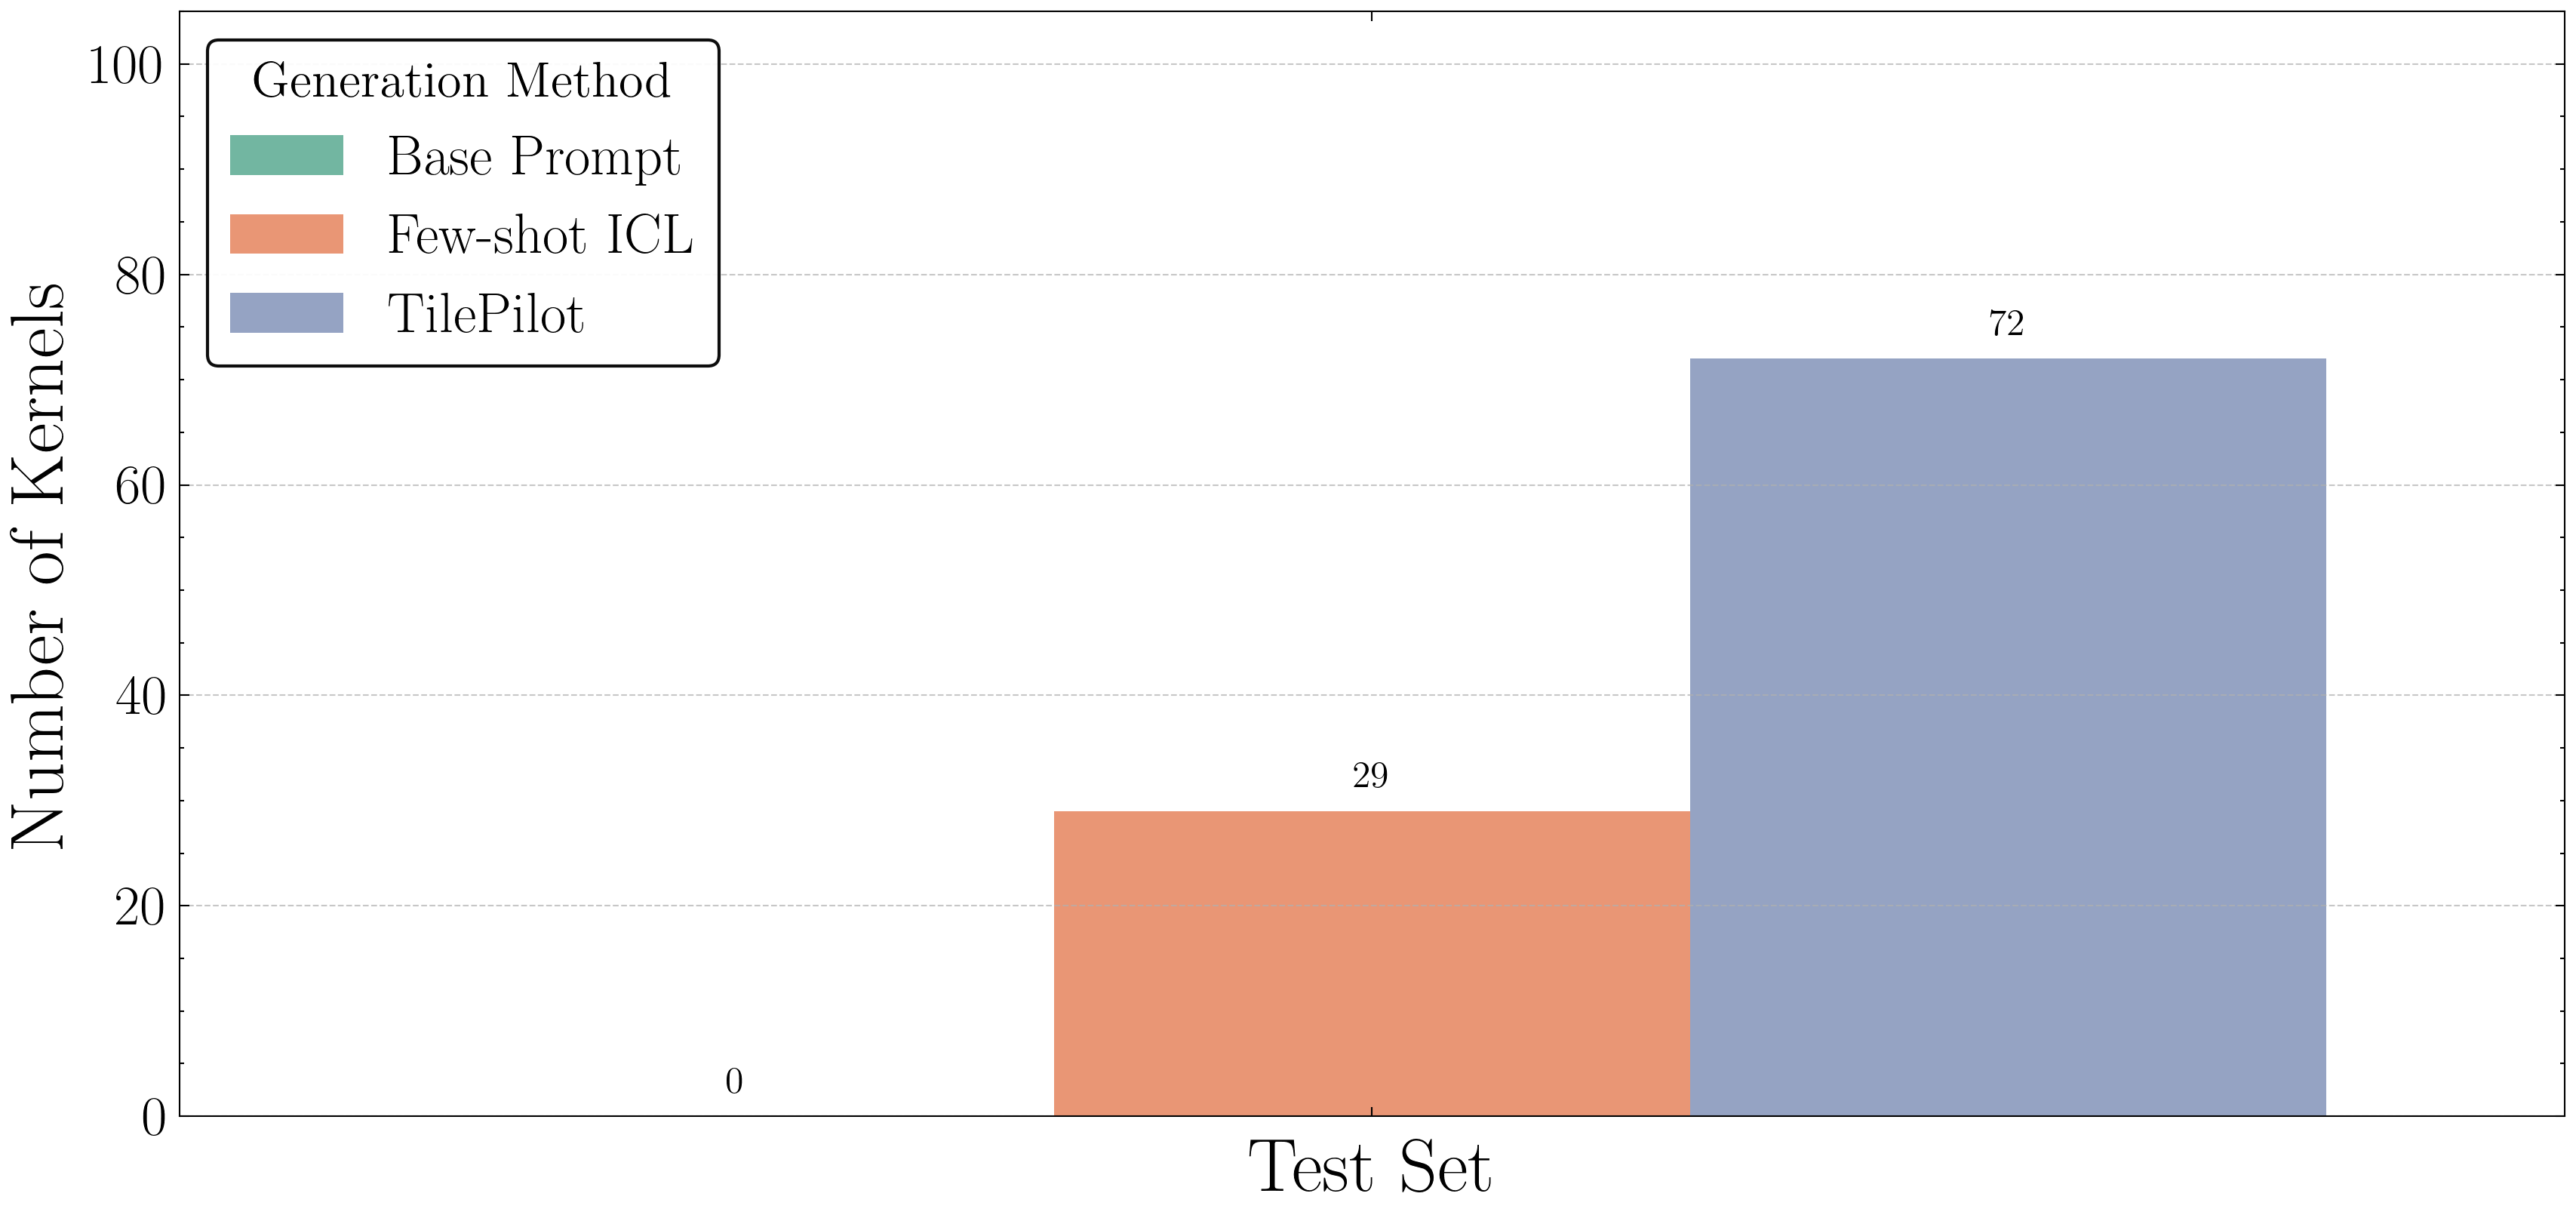
\includegraphics[width=0.8\textwidth]{plots/kernel_success_rate_test_set.png}
    \caption{Test set success rates across generation methods. TilePilot achieves substantial improvements in zero-shot generalization compared to baseline approaches.}
    \label{fig:test_set_success}
\end{figure}

\textbf{Performance Analysis:} More importantly, TilePilot achieved exceptional performance on the test set with a mean speedup of 1.25x compared to PyTorch baselines. Remarkably, 69\% of generated kernels (50 out of 72) outperformed their PyTorch equivalents, with speedups ranging up to 13.1x. Figure~\ref{fig:test_set_speedup} shows the distribution of speedup ratios across the test set, highlighting both the consistency and the potential for significant performance improvements.

\begin{figure}[htbp]
    \centering
    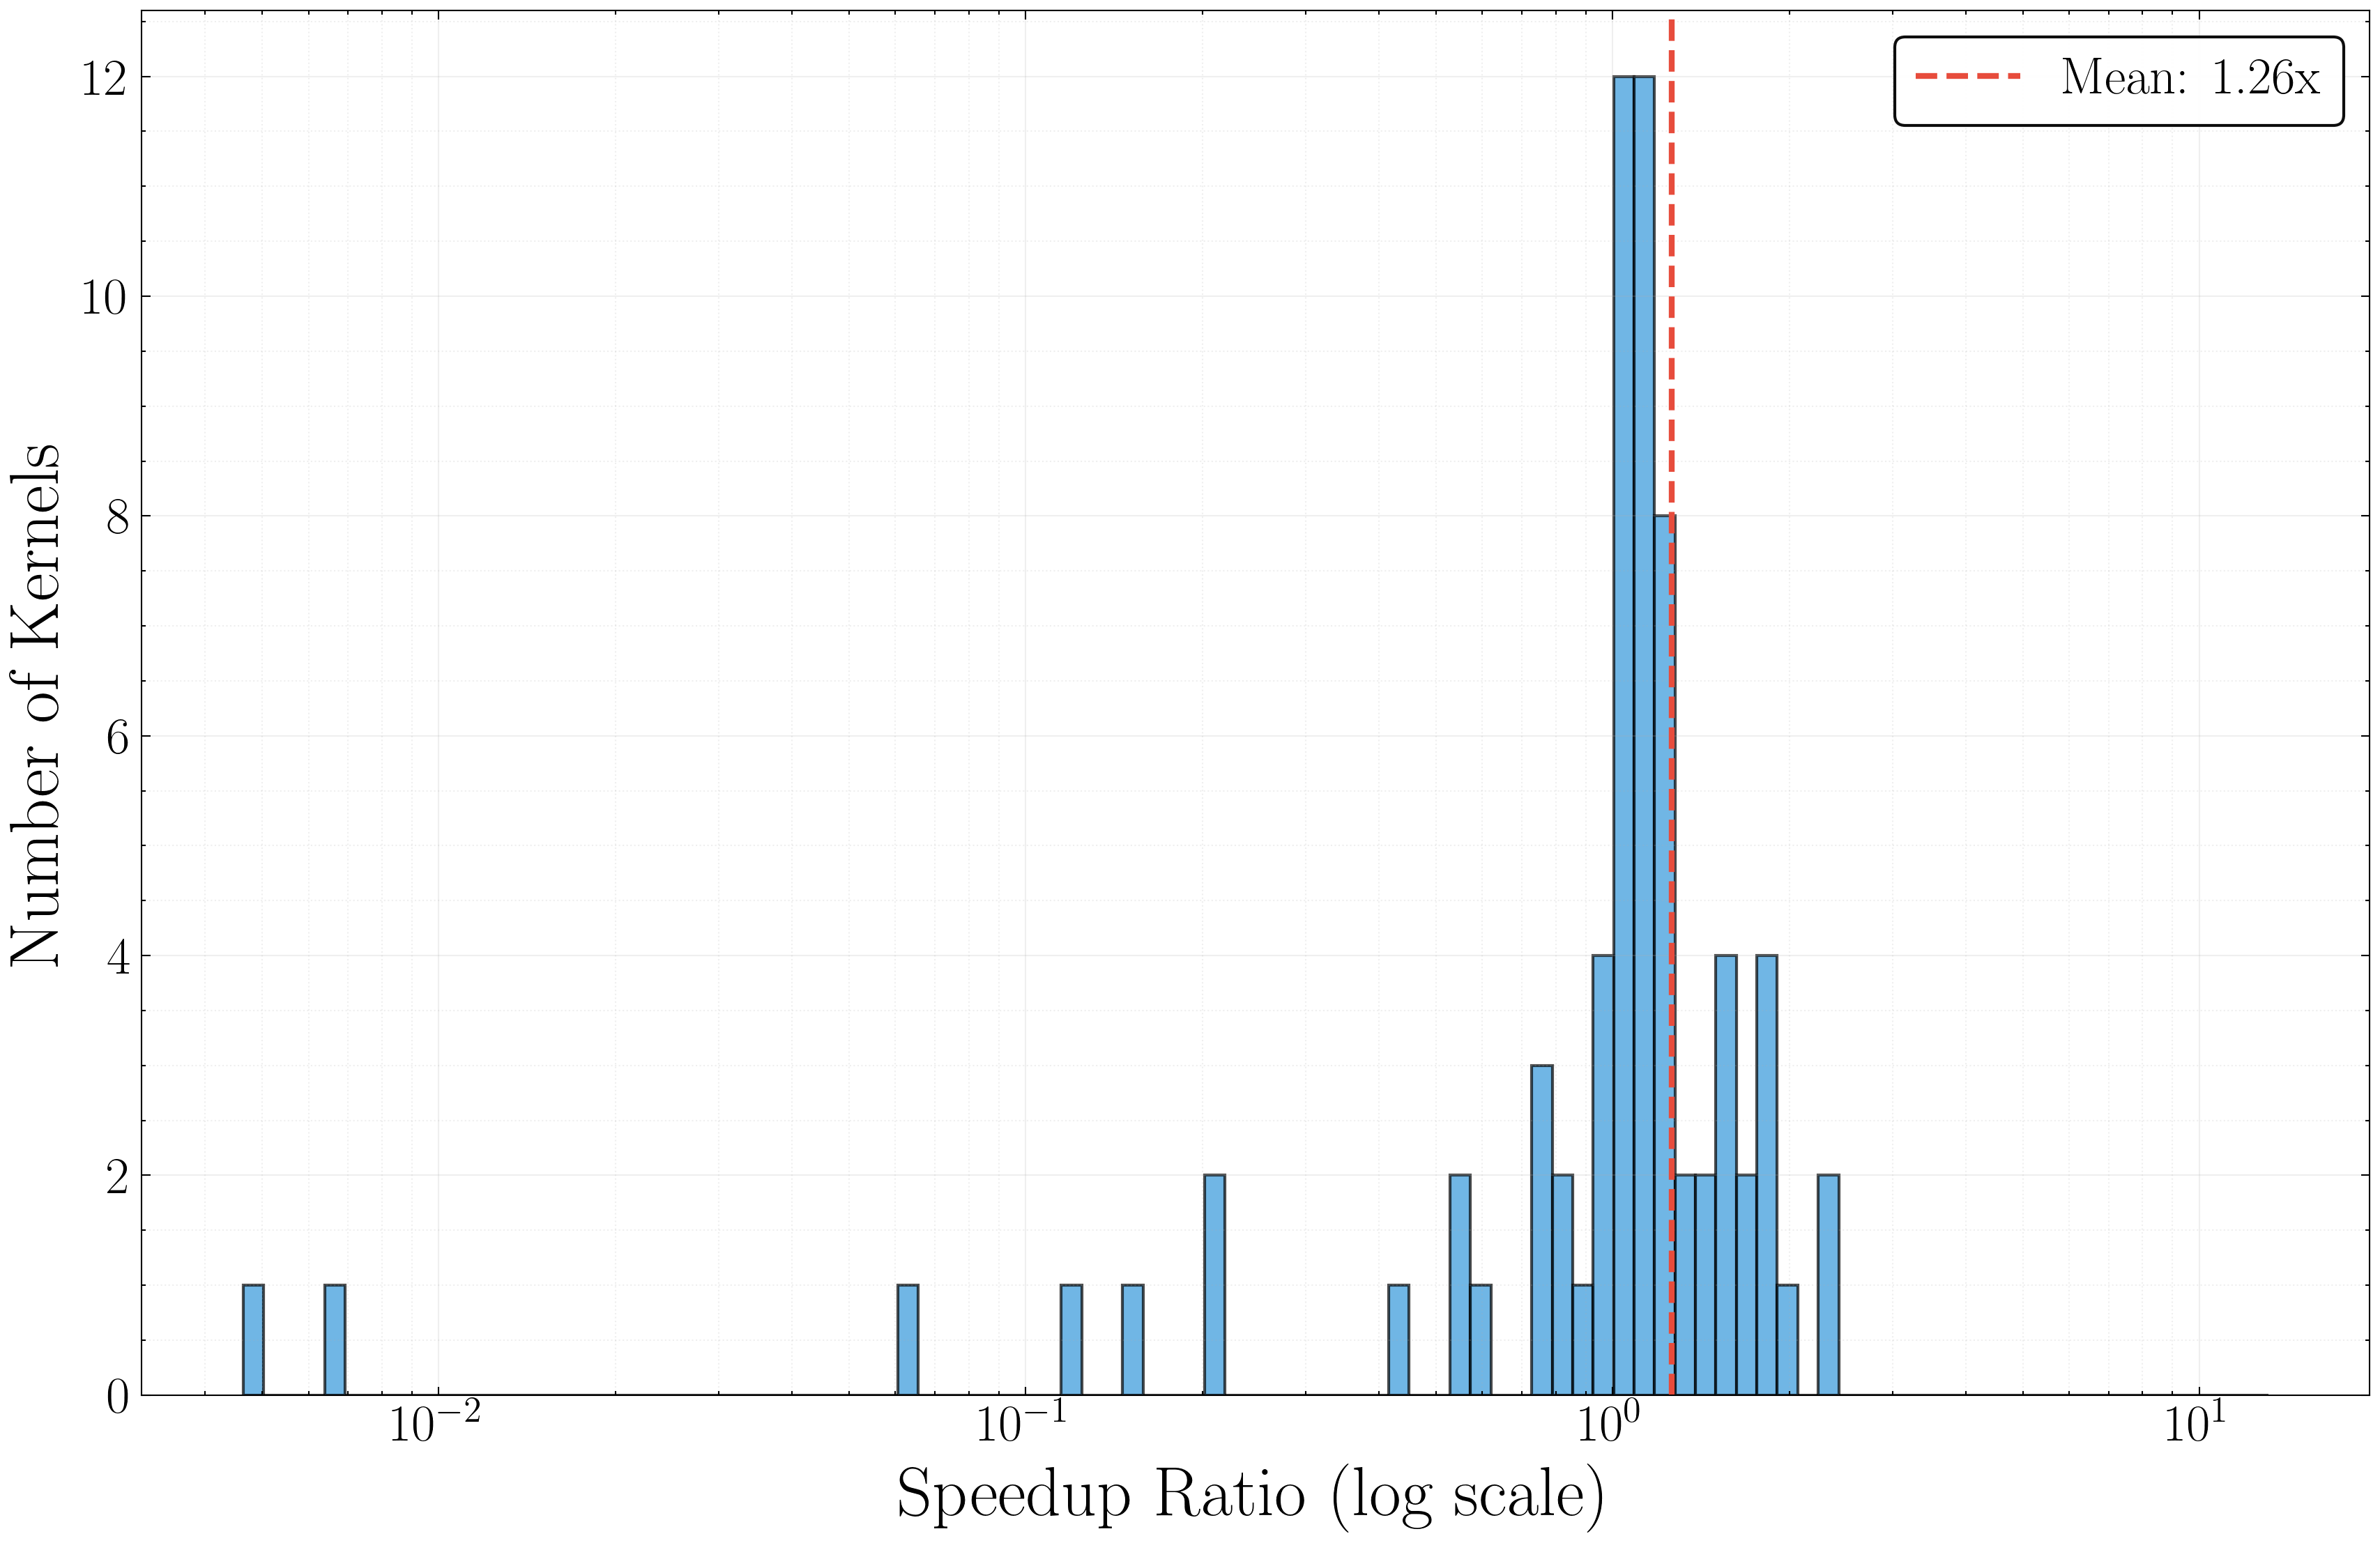
\includegraphics[width=0.8\textwidth]{plots/speedup_distribution_testset.png}
    \caption{Distribution of speedup ratios for test set kernels (log scale). The red vertical line indicates the mean speedup of 1.25x, showing that the majority of kernels achieve meaningful performance improvements over PyTorch baselines.}
    \label{fig:test_set_speedup}
\end{figure}

These test set results validate several key aspects of our approach: (1) the knowledge retrieval mechanism successfully generalizes to unseen problems, (2) the patterns learned from our seed kernels are broadly applicable across diverse optimization scenarios, and (3) the performance benefits observed on the training data translate effectively to new, unseen challenges. The strong test set performance provides confidence that TilePilot represents a robust and practical solution for automated GPU kernel generation.

\section{Analysis}

\subsection{Why RAG Succeeds}

The dramatic improvement enabled by RAG demonstrates several key insights:

1. \textbf{Pattern Matching:} Analysis of successful Level 2 kernels reveals that the vast majority of kernels involve variations of patterns present in our knowledge base. For instance, the matrix multiplication followed by element-wise operations pattern was consistently retrieved and adapted for similar fusion patterns. We believe we can further improve our success rate by creating more tuned handwritten examples for common patterns.

2. \textbf{Context Specificity:} Unlike fixed few-shot examples, RAG provides task-specific context. When generating convolution kernels, the system retrieved similar convolution implementations with implicit GEMM and similar tiling patterns, leading to better architectural choices compared to naive few-shot ICL.

3. \textbf{Knowledge Base Growth:} Since we build our knowledge base from the set of correct generated kernels, we effectively have a self-evolving knowledge base that is constantly growing and improving. This creates a positive feedback loop that can allow the system to adapt to new patterns and optimizations over time.

\subsection{Mathematical Optimization Discovery}

A particularly significant finding was TilePilot's ability to act as an LLM compiler, discovering mathematical optimizations that reduce algorithmic complexity. This capability demonstrates that by leveraging the priors of large language models, our system can extend beyond simple pattern matching to sophisticated reasoning.

In KernelBench Level 2 Problem 14, instead of implementing the naive sequence:
$$
X \rightarrow X \cdot W^T \rightarrow \text{divide by 2} \rightarrow \text{sum}(\text{dim}=1) \rightarrow \text{scale}
$$
The system recognized the mathematical equivalence and implemented:
$$
\text{sum}(X \cdot W^T, \text{dim}=1) = X \cdot \text{sum}(W, \text{dim}=0)
$$
This optimization reduced computational complexity from $O(\text{batch} \times \text{input} \times \text{hidden})$ to $O(\text{batch} \times \text{input})$, allowing us to achieve a significant speedup.

Another striking example of mathematical optimization occurred in Level 2 Problem 13. The original computational graph consisted of the following operations:
$$
X \rightarrow \text{ConvTranspose3d} \rightarrow \text{Mean} \rightarrow \text{Add Bias} \rightarrow \text{Softmax} \rightarrow \text{Tanh} \rightarrow \text{Scale}
$$
TilePilot recognized that this sequence simplifies dramatically. After taking the mean over spatial dimensions and applying softmax to a single value (which always outputs 1.0), the entire pipeline reduces to $\tanh(1.0) \times \text{scale}$. The generated kernel essentially compiles away the entire complex operation sequence, replacing it with a simple constant fill operation. This optimization represents complete algorithmic elimination rather than just computational efficiency improvements, though it may also highlight limitations in KernelBench's evaluation framework where such extreme mathematical simplifications are possible.

\subsection{Performance Limitations Analysis}

Our analysis identifies four primary factors limiting performance:

\textbf{Memory Access Patterns:} In many underperforming kernels, we observed inefficient memory coalescing patterns that were suboptimal for our target hardware. This limitation was particularly pronounced in Level 1 tasks, where PyTorch's vendor-optimized implementations proved challenging to surpass without extensive hardware-specific tuning.

\textbf{Thread Block Configuration:} Our manual analysis of 20 slow-performing kernels revealed that 60\% suffered from suboptimal thread block size configurations. The current implementation lacks a systematic approach to exploring the thread configuration space, which is crucial for achieving optimal performance. TileLang does offer an autotuning system that works well for simple kernels, but the feature is very experimental and slow. We believe the incorporation of this feature in the future once it matures will be a major improvement.

\textbf{Knowledge Base Gaps:} The relatively modest performance improvement in Level 3 (28\% above baseline) can be attributed to gaps in our knowledge base, particularly regarding advanced optimization techniques such as multi-kernel fusion and custom scheduling strategies.

\textbf{Evaluation Framework Issues:} The default input sizes for KernelBench are often too small, causing the benchmark to measure the kernel-launch overhead more than the actual kernel execution time. In some cases, it causes efficient kernels to crash because the input size is too small for the Tensor Memory Accelerator (TMA) in the H100. We manually enlarged the input sizes of tasks that crashed, but we believe the real speedup may be higher once these input sizes are fixed. We spoke to the authors of KernelBench and they were aware of this issue and are working on a fix.

\subsection{Failure Cases}

We also conducted an analysis of failure modes in our current system:

\textbf{Complex Scheduling:} Level 3 failures primarily involve kernels requiring sophisticated scheduling that exceeds current LLM reasoning capabilities about hardware resource management.

\textbf{Numerical Stability:} 8\% of failures involved numerically unstable implementations that passed individual tests but failed on edge cases with extreme input values.

\textbf{TileLang Syntax:} 15\% of failures were due to subtle TileLang syntax errors, often involving incorrect tensor dimension handling or memory layout specifications.

% ---------------- KTO SECTION ----------------
\section{Application of TilePilot: KTO Training}

\subsection{Post-hoc Reasoning Trace Generation}

We wanted to test if TilePilot’s own verified outputs teach a much smaller (8B) open-weight model to generate high-quality GPU kernels. To do this, we developed an approach that combines our successful and correct kernel generations with post-hoc reasoning traces where we have strong models look at the correct answer plus the problem and generate a reasoning trace to go from problem to answer. After generating our initial collection of 214 verified kernels, we created detailed reasoning traces explaining the generation process for each successful kernel.

\textbf{Reasoning Trace Construction:} For each successful kernel in our collection, we prompted GPT-4 to generate step-by-step reasoning traces that explain:
\begin{itemize}
\item The mapping from PyTorch operations to TileLang constructs
\item Key optimization decisions (memory access patterns, thread organization, operator fusion)
\item Mathematical transformations and algorithmic insights
\item Performance considerations and trade-offs
\end{itemize}

We intend for these reasoning traces to serve as high-quality training examples that capture not just the final kernel implementation, but the underlying problem-solving process that leads to successful GPU kernel optimization.

\subsection{Preference Optimization}

Due to our limited dataset, we decided to try Kahneman-Tversky Optimization (KTO)~\cite{ethayarajh2024ktomodelalignmentprospect} to train our model on the reasoning trace dataset. KTO is a preference optimization technique based on prospect theory that can work with unpaired preference data, making it particularly suitable for our domain where obtaining paired comparisons is expensive. It is also an algorithm that effectively uses negative examples, which we had a lot of. 

\textbf{Dataset Construction:} Our KTO dataset consists of 2,400 examples structured as follows:
\begin{itemize}
\item \textbf{Prompt:} PyTorch operation specification with detailed requirements
\item \textbf{Chosen:} Successful kernel implementation with post-hoc reasoning trace generated by a stronger model
\item \textbf{Rejected:} Failed or suboptimal reasoning traces generated by the base model
\end{itemize}

The reasoning traces provide rich contextual information that helps the model learn the underlying patterns and decision-making processes required for effective kernel generation.

\textbf{Training Configuration:} We fine-tuned the Seed-Coder-8B-Instruct model using KTO with the following configuration:
\begin{itemize}
\item \textbf{Learning Rate:} $1 \times 10^{-6}$ (within KTO's recommended range for $\beta = 0.1$)
\item \textbf{Batch Size:} Effective batch size of 32 (per-device batch size of 2, gradient accumulation steps of 2, across 8 GPUs)
\item \textbf{Training Duration:} 10 epochs over the 2,400-sample dataset
\item \textbf{KTO Parameters:} $\beta = 0.1$, equal weighting for desirable and undesirable examples
\end{itemize}


\subsection{KTO Results}

We found that training our 8B language model with KTO did not yield meaningful improvements in \texttt{pass@5} on our held-out test set. While we successfully augmented our dataset with multiple reasoning traces per KernelBench task, we hypothesize that two factors limited performance: the narrow task distribution and the capacity of the base model itself. Despite reinforcement on high-quality examples, the 8B model may lack the inductive biases and representational power required to generalize effective optimization strategies across diverse CUDA tasks. In future work, we plan to investigate scaling KTO to stronger base models, such as 32B models to better capture the complexity of kernel optimization.

\begin{table}[h]
\centering
\begin{tabular}{lrrrr}
\toprule
\textbf{Run} & \textbf{Correct} & \textbf{Compile Errors} & \textbf{Correctness Errors} & \textbf{pass@5} \\
\midrule
Before & 0 & 456 & 203 & 0.00 \\
After  & 1 & 408 & 178 & 0.01 \\
\bottomrule
\end{tabular}
\caption{Comparison of the two runs before and after KTO training. Compiler errors includes actual compiler errors and malformed file generations.}
\end{table}


% \% ---------------- END KTO SECTION ----------------

\section{Conclusion}

TilePilot demonstrates that retrieval-augmented generation can dramatically outperform expensive sampling strategies for GPU kernel optimization. Our approach achieves a 78\% improvement in success rates over few-shot methods while reducing costs by 50x compared to brute-force approaches (\$0.30 vs \$15.00 per successful kernel). The robustness of our approach is further validated by strong performance on a held-out test set, where TilePilot generated 72 successful kernels with a mean speedup of 1.25x, demonstrating effective generalization to unseen problems.

The key insight is validated by our results: Level 2 tasks involving operator fusion show exceptional performance with 58\% of kernels outperforming PyTorch baselines and achieving an average speedup of 1.26x. Most significantly, TilePilot exhibits emergent compiler-like behavior, discovering mathematical optimizations that reduce algorithmic complexity rather than merely translating operations. This suggests that LLMs can serve as sophisticated optimization engines when provided with appropriate domain knowledge and retrieval mechanisms.

Our work establishes retrieval-augmented generation as a viable paradigm for specialized code generation tasks, with broader implications for AI-assisted optimization in domains characterized by pattern recombination, limited training data, and high performance sensitivity.

\section{Team Responsibilities}

\textbf{Jack Le:} Designed and implemented the core RAG system architecture and progressive learning framework. Developed the knowledge retrieval components and embedding-based similarity search. Conducted the speedup performance analysis and led the investigation of LLM compiler-like optimizations such as the case study.

\textbf{Nathan Paek:} Implemented the multi-turn optimization system for iterative kernel improvement. Conducted comprehensive failure case analysis and evaluation framework assessment, including modifying KernelBench to work with TileLang. Generated the KTO dataset and conducted evaluation for baseline and fine-tuned models. Responsible for experimental setup, hardware configuration, and baseline method implementations.

\textbf{William Li:} Implemented the in-context learning pipeline and conducted detailed correctness studies. Developed and ran the full distributed training pipeline and checkpointing for KTO training. Led the investigation into why RAG succeeds through pattern matching and context specificity analysis. Built pipeline to generate diverse reasoning strategies used in training and evaluation. \\


\textbf{All team members:} Wrote the report and created the presentation, collaboratively created the initial seed kernel collection of 37 high-quality TileLang implementations that served as the foundation for our knowledge base.

{\small
\bibliography{sample}
}

\end{document}